\documentclass[10pt]{beamer}
\mode<presentation> {
\usepackage[utf8]{inputenc}
\usetheme{Berlin}

%\usecolortheme{seahorse}
\usepackage{multicol}
\usepackage{adjustbox,lipsum}
\usepackage{booktabs}
\usepackage[scale=2]{ccicons}
\usepackage{longtable}
\usepackage{xcolor}

\usepackage{array}
\usepackage{makecell}
\usepackage{amsmath}
\usepackage{graphicx}
\newcommand{\bn}[1]{{\fontseries{b}\selectfont#1}}
\usepackage{siunitx}

\usepackage[percent]{overpic}
\usepackage{pgfplots}
\pgfplotsset{compat=1.18}
\usepgfplotslibrary{dateplot}
\usepackage{pifont}

\usepackage{arydshln}
\usepackage{xspace}
\usepackage{eurosym}
\usepackage[labelformat=empty]{caption}
\usepackage{appendixnumberbeamer}
\usepackage{hyperref}
\usepackage{lipsum}
\usepackage{adjustbox}

\newcommand{\dimtorightedge}{%
  \dimexpr\paperwidth-1in-\hoffset-\oddsidemargin\relax}
\newcommand{\dimtotop}{%
  \dimexpr\height-1in-\voffset-\topmargin-\headheight-\headsep\relax}

\usepackage{float}
\usepackage[backend=bibtex, maxcitenames=1, style=authoryear, doi=false, isbn=false, url=false]{biblatex}
\addbibresource{bibliography.bib}
\setbeamertemplate{bibliography item}{}

\usepackage{ragged2e}

\definecolor{metured}{RGB}{227, 24, 55}
\definecolor{metugray}{RGB}{113, 112, 115}
\definecolor{metublack}{RGB}{20, 16, 6}
\definecolor{metugreen}{RGB}{0, 130, 101}
\definecolor{metubrown}{RGB}{122, 111, 0}
\definecolor{metublue}{RGB}{0, 92, 171}

\hypersetup{
    colorlinks=metublue,
    linkcolor=metublue,
    urlcolor=metublue,
    citecolor=metublue
}
\usecolortheme[named=metublue]{structure}
\usepackage{tikz}
\usetikzlibrary{positioning, shapes.geometric, fit, backgrounds, calc, arrows.meta}
\def\indicatrice{\textrm{1\kern-0.25emI}}
\setbeamertemplate{navigation symbols}{}

\setbeamertemplate{headline}
{%
  \begin{beamercolorbox}[colsep=1.5pt]{upper separation line head}
  \end{beamercolorbox}
  \begin{beamercolorbox}{section in head/foot}
    \vskip2pt\insertnavigation{\paperwidth}\vskip2pt
  \end{beamercolorbox}%
  \begin{beamercolorbox}[colsep=1.5pt]{lower separation line head}
  \end{beamercolorbox}
}

\usepackage[most]{tcolorbox}
}
\newenvironment{quadfont}[2]{\begingroup\fontsize{#1}{#2}\selectfont}{\endgroup}


\author{Alexander Csek\"{o}\textsuperscript{}}

\titlegraphic{
  
\includegraphics[height=1.5cm]{figures/TU_Logo.pdf}
  \hfill
  
\includegraphics[height=1.5cm]{figures/EEG_logo.png}
}

\institute{\textsuperscript{}Energy Economics Group (EEG), Technische Universität Wien, Vienna, Austria}
\date{\today}

\usepackage[utf8]{inputenc}
\usepackage{tikz}
\usepackage[most]{tcolorbox}

% Define the custom green color from your reference image
\definecolor{eegGreen}{RGB}{56, 114, 27}

% Remove default navigation symbols and header/footer for the title slide
\setbeamertemplate{navigation symbols}{}




%------------------------------------------------
% Opening
%------------------------------------------------


%------------------------------------------------
\begin{document}
%------------------------------------------------

\begin{frame}
    \centering

    % --- Top Title Block ---
    \begin{tcolorbox}[
        enhanced,
        colback=metublue,
        colframe=metublue,
        arc=0mm,
        width=0.85\textwidth,
        boxrule=0pt,
        center,
        halign=center,
        valign=center,
        height=2.5cm
    ]
        \color{white}
        {\Large Strategic Allocation of Battery Energy Storage Systems} \\
        \vspace{0.2cm}
        {\large in Multi-Service Markets: An EPEC Modeling Approach}
    \end{tcolorbox}

    \vspace{0.8cm}

    % --- Authors (Standard size) ---
    {Alexander Csek\"{o}$^{1}$, Daniel Horvath$^{1}$, Johann Auer$^{1}$, Sebastian Zwickl-Bernhard$^{1}$}

    \vspace{0.6cm}

    % --- Affiliations ---
    \scriptsize
    $^1$Energy Economics Group (EEG), Technische Universität Wien (TU Wien)

    \vspace{0.4cm}

    % --- Date ---
    {\normalsize \today}

    \vspace{0.8cm}

    % --- Logos ---
    \begin{columns}[c]
        \column{0.4\textwidth}
        \centering
        
\includegraphics[height=1.2cm, keepaspectratio]{figures/TU_Logo.pdf}

        \column{0.4\textwidth}
        \centering
        
\includegraphics[height=1.2cm, keepaspectratio]{figures/EEG_logo.png}
    \end{columns}

\end{frame}


\begin{frame}{Start and Current State}
\vspace{0.2cm}

\begin{itemize}
    \item 8 July 2026
    \item \textbf{Problem:} we need to validate and expand the model -- some suspicion because of the fast convergence of the Gauss--Seidel algorithm
    \item \textbf{Problem:} the aFRR market looks very attractive
\end{itemize}

\vspace{0.3cm}
\small
\begin{table}
    \centering
    \begin{tabular}{lccc}
        \toprule
        \textbf{Investor} & \textbf{WACC} & \textbf{Arbitrage (\euro)} & \textbf{aFRR (\euro)} \\
        \midrule
        Investor 1 & 8.0\%  & -2,574.26 & 332,852.44 \\
        Investor 2 & 12.0\% & 4,521.00  & 292,986.68 \\
        Investor 3 & 15.0\% & 3,759.11  & 293,034.14 \\
        Investor 4 & 20.0\% & 3,532.13  & 293,041.04 \\
        \bottomrule
    \end{tabular}
    \caption{Multi-service scenario: daily arbitrage vs.\ aFRR revenue.}
\end{table}
\vspace{0.2cm}

\begin{itemize}
    \item \textbf{Goal:} robust results from an extended model by end of September (Alex)
\end{itemize}
\end{frame}

\begin{frame}{Resolution: Treat aFRR Activation as Uncertainty}
\vspace{0.05cm}

\small
\begin{itemize}
    \item The old model rewards aFRR capacity, but does not fully price the \textbf{energy consequence} of activation.
    \item New plan: keep 24 hours and the same 5-node grid, but solve the LLP over activation scenarios \(s \in \mathcal{S}\).
    \item Example scenarios: no activation, up-heavy, down-heavy, mixed, each with probability \(\omega_s\).
    \item The key correction is in the nodal energy balance, where the nodal price \(\lambda_{n,t,s}\) emerges.
\end{itemize}

\vspace{0.15cm}
\footnotesize
\begin{align*}
\sum_{g \in G_n} P_{g,t,s}
&+ \sum_i \Big(
P^{discharge}_{i,n,t,s}
- P^{charge}_{i,n,t,s}
\textcolor{metublue}{+ P^{aFRR,up}_{i,n,t,s}
- P^{aFRR,down}_{i,n,t,s}}
\Big) \\
&\quad
 + P^{shed}_{n,t,s}
 - D^{el}_{n,t}
 = NetInjection_{n,t,s},
 \qquad \forall n,t,s
 \quad (\lambda_{n,t,s})
\end{align*}

\vspace{0.05cm}
\footnotesize
\begin{align*}
\textcolor{metublue}{\sum_{i,n} R^{aFRR}_{i,n,b} + P^{aFRR,def}_{b}}
&\textcolor{metublue}{\geq D^{aFRR}_{b}},
\qquad \textcolor{metublue}{\forall b}
\quad \textcolor{metublue}{(\lambda_{aFRR,b})}
\end{align*}

\end{frame}



\begin{frame}{Meeting Outcome}
\vspace{0.2cm}

\begin{itemize}
    \item No aFRR, only spot market
    \item \textbf{Core challenge:} model initial distribution and competition for power at nodes
    \item Use different investors that differ in battery operation
    \item Next meeting: mid August - preliminary results required!
\end{itemize}

\end{frame}


\begin{frame}{Network Revision (15 July 2026)}
\vspace{0.2cm}

\begin{itemize}
    \item \textbf{Christoph suggested revising the network} so that price signals are more meaningful
    \item \textbf{Confirmed:} current calibration produces heavy congestion in every high-demand hour (line limits L12/L45 saturate at 100\% utilization, nodal prices spike to \euro{}2,000--4,000/MWh)
    \item \textbf{Plan:} loosen the transmission network so it is less binding by default, and increase PV capacity so midday prices show a visible low-price trough
\end{itemize}

\end{frame}


\begin{frame}{IEEE-9 calibration: two renewable export bottlenecks}
\vspace{-0.15cm}

\begin{columns}[T,onlytextwidth]
    \column{0.60\textwidth}
    \centering
    \resizebox{\linewidth}{!}{%
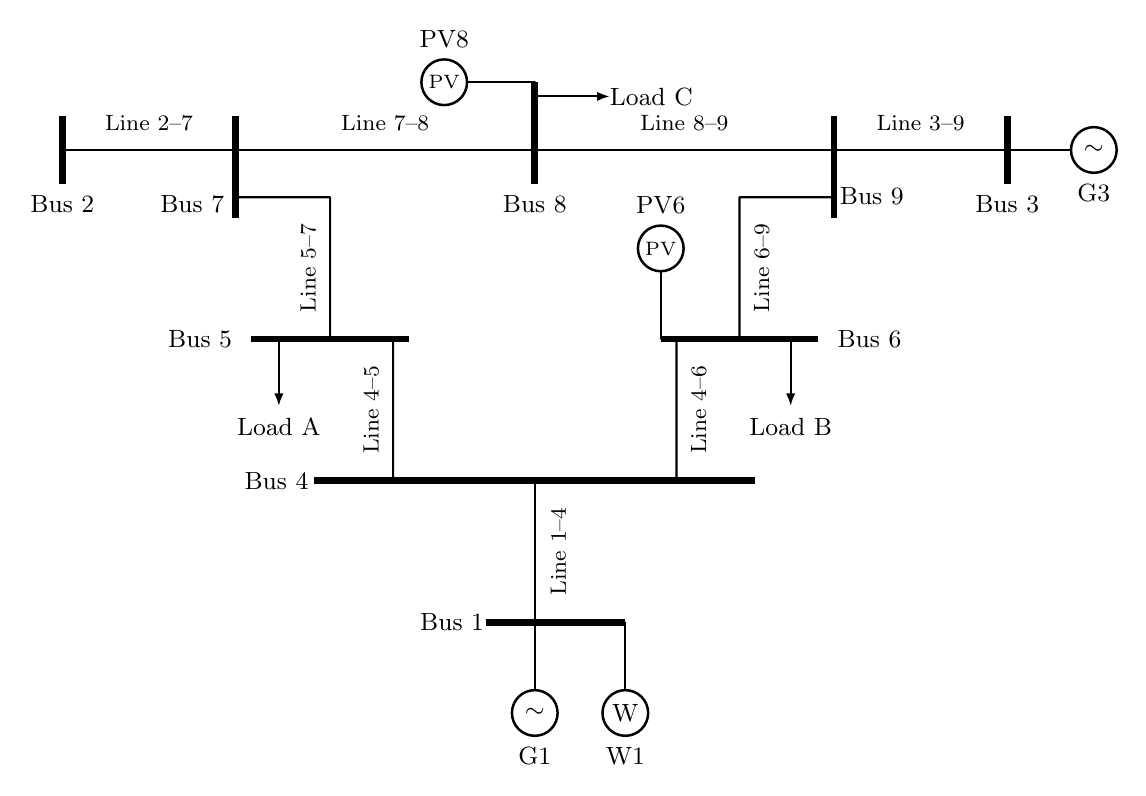
\begin{tikzpicture}[
  x=1cm,
  y=1cm,
  transmission/.style={
    draw=black,
    line width=0.75pt,
    line cap=round,
    line join=round
  },
  crossing/.style={
    transmission,
    preaction={draw=white,line width=3.0pt,line cap=round}
  },
  busbar/.style={
    draw=black,
    line width=2.4pt,
    line cap=butt
  },
  bus label/.style={
    font=\small,
    inner sep=1pt
  },
  line label/.style={
    font=\footnotesize,
    fill=white,
    inner sep=1.2pt
  },
  generator/.style={
    circle,
    draw=black,
    fill=white,
    line width=0.9pt,
    minimum size=0.58cm,
    inner sep=0pt,
    font=\small
  },
  load arrow/.style={
    draw=black,
    line width=0.75pt,
    -{Latex[length=4.5pt,width=3.4pt]}
  },
  component label/.style={
    font=\small,
    inner sep=1pt
  }
]

% ---------------------------------------------------------------------------
% Adjustable bus coordinates, arranged to match the reference skeleton.
% The upper buses are vertical; the middle and lower buses are horizontal.
% ---------------------------------------------------------------------------
\coordinate (n2) at (-6.00, 3.00);
\coordinate (n7) at (-3.80, 3.00);
\coordinate (n8) at ( 0.00, 3.00);
\coordinate (n9) at ( 3.80, 3.00);
\coordinate (n3) at ( 6.00, 3.00);
\coordinate (n5) at (-2.60, 0.60);
\coordinate (n6) at ( 2.60, 0.60);
\coordinate (n4) at ( 0.00,-1.20);
\coordinate (n1) at ( 0.00,-3.00);

% Generator symbol coordinates.
% Bus 2 has no generator in the calibrated dataset (G_IEEE2 removed).
\coordinate (g3) at ( 7.10, 3.00);
\coordinate (g1) at ( 0.00,-4.15);

% Renewable generator symbol coordinates: wind at Bus 1, PV at Buses 6 and 8.
% Each sits on a stub drawn normal (perpendicular) to its own busbar.
\coordinate (w1) at ( 1.15,-4.15);
\coordinate (pv6) at ( 1.60, 1.75);
\coordinate (pv8) at (-1.15, 3.86);

% ---------------------------------------------------------------------------
% Transmission connections (drawn before the busbars)
% ---------------------------------------------------------------------------

% Upper spine and the two outer links.
\draw[transmission] (n2) -- (n7); % N2--N7
\draw[transmission] (n7) -- (n8); % N7--N8
\draw[transmission] (n8) -- (n9); % N8--N9
\draw[transmission] (n9) -- (n3); % N9--N3

% Left and right descending sides of the reference skeleton.
\draw[transmission]
  (n5) -- (-2.60,2.40) -- ($(n7)+(0,-0.60)$); % N7--N5
\draw[transmission]
  ($(n5)+(0.80,0)$) -- ($(n4)+(-1.80,0)$); % N5--N4
\draw[transmission]
  ($(n4)+(1.80,0)$) -- ($(n6)+(-0.80,0)$); % N4--N6
\draw[transmission]
  (n6) -- ( 2.60,2.40) -- ($(n9)+(0,-0.60)$); % N6--N9

% Lower central link; transformer symbols are intentionally omitted.
\draw[transmission] (n4) -- (n1); % N4--N1

% Generator connections.
\draw[transmission] (n3) -- (g3);
\draw[transmission] (n1) -- (g1);

% Renewable generator connections: each stub is normal to its own busbar.
\draw[transmission] ($(n1)+(1.15,0)$) -- (w1);
\draw[transmission] ($(n6)+(-1.00,0)$) -- (pv6);
\draw[transmission] ($(n8)+(0,0.86)$) -- (pv8);

% Load connections: C at Bus 8, A at Bus 5, and B at Bus 6.
\draw[load arrow]
  ($(n8)+(0,0.68)$) -- ($(n8)+(0.95,0.68)$);
\draw[load arrow]
  ($(n5)+(-0.65,0)$) -- ($(n5)+(-0.65,-0.85)$);
\draw[load arrow]
  ($(n6)+(0.65,0)$) -- ($(n6)+(0.65,-0.85)$);

% ---------------------------------------------------------------------------
% Busbars (drawn last so they remain visually dominant)
% ---------------------------------------------------------------------------

% Standard vertical busbars at the two outer buses.
\foreach \bus in {n2,n3}{
  \draw[busbar]
    ($(\bus)+(0,-0.43)$) -- ($(\bus)+(0,0.43)$);
}

% Bus 8 extends farther in the positive y direction.
\draw[busbar] ($(n8)+(0,-0.43)$) -- ($(n8)+(0,0.86)$);

% Buses 7 and 9 extend farther in the negative y direction.
\foreach \bus in {n7,n9}{
  \draw[busbar]
    ($(\bus)+(0,-0.86)$) -- ($(\bus)+(0,0.43)$);
}

% Buses 5 and 6 extend equally in both x directions.
\foreach \bus in {n5,n6}{
  \draw[busbar]
    ($(\bus)+(-1.00,0)$) -- ($(\bus)+(1.00,0)$);
}

% Bus 4 spans beneath Buses 5 and 6 so both connections can be vertical.
\draw[busbar] ($(n4)+(-2.80,0)$) -- ($(n4)+(2.80,0)$);

% Bus 1 extends farther in the positive x direction for the wind-generator stub.
\draw[busbar] ($(n1)+(-0.62,0)$) -- ($(n1)+(1.15,0)$);

% ---------------------------------------------------------------------------
% Bus names
% ---------------------------------------------------------------------------
\node[bus label] at ($(n2)+(0,-0.68)$) {Bus 2};
\node[bus label] at ($(n7)+(-0.55,-0.68)$) {Bus 7};
\node[bus label] at ($(n8)+(0,-0.68)$) {Bus 8};
\node[bus label] at ($(n9)+(0.48,-0.58)$) {Bus 9};
\node[bus label] at ($(n3)+(0,-0.68)$) {Bus 3};
\node[bus label] at ($(n5)+(-1.65,0)$) {Bus 5};
\node[bus label] at ($(n6)+( 1.65,0)$) {Bus 6};
\node[bus label] at ($(n4)+(-3.28,0)$) {Bus 4};
\node[bus label] at ($(n1)+(-1.05,0)$) {Bus 1};

% ---------------------------------------------------------------------------
% Line names
% ---------------------------------------------------------------------------
\node[line label] at (-4.90,3.34) {Line 2--7};
\node[line label] at (-1.90,3.34) {Line 7--8};
\node[line label] at ( 1.90,3.34) {Line 8--9};
\node[line label] at ( 4.90,3.34) {Line 3--9};
\node[line label,rotate=90] at (-2.88,1.50) {Line 5--7};
\node[line label,rotate=90] at (-2.08,-0.30) {Line 4--5};
\node[line label,rotate=90] at ( 2.08,-0.30) {Line 4--6};
\node[line label,rotate=90] at ( 2.88,1.50) {Line 6--9};
\node[line label,rotate=90] at ( 0.30,-2.10) {Line 1--4};

% Synchronous-generator symbols and names.
\node[generator] at (g3) {$\sim$};
\node[generator] at (g1) {$\sim$};
\node[component label] at ($(g3)+(0,-0.55)$) {G3};
\node[component label] at ($(g1)+(0,-0.55)$) {G1};

% Renewable-generator symbols and names (same circle as the synchronous units).
\node[generator] at (w1) {W};
\node[generator,font=\scriptsize] at (pv6) {PV};
\node[generator,font=\scriptsize] at (pv8) {PV};
\node[component label] at ($(w1)+(0,-0.55)$) {W1};
\node[component label] at ($(pv6)+(0,0.55)$) {PV6};
\node[component label] at ($(pv8)+(0,0.55)$) {PV8};

% Load names.
\node[component label] at ($(n8)+(1.48,0.68)$) {Load C};
\node[component label] at ($(n5)+(-0.65,-1.12)$) {Load A};
\node[component label] at ($(n6)+( 0.65,-1.12)$) {Load B};

\end{tikzpicture}%
}

    \column{0.40\textwidth}
    \vspace{0.05cm}
    {\scriptsize
    \begin{tabular}{@{}lccc@{}}
        \toprule
        \textbf{Unit} & \textbf{Node} & \textbf{MW} & \textbf{MC} \\
        & & & \textbf{\euro/MWh} \\
        \midrule
        G1 & N1 & 250 & 60.00 \\
        G2 & N2 & 300 & 52.20 \\
        G3 & N3 & 270 & 67.15 \\
        Wind & N1 & 105 & 0.00 \\
        PV & N6 & 235 & 0.00 \\
        PV & N8 & 436 & 0.00 \\
        \bottomrule
    \end{tabular}}
\end{columns}
\end{frame}


\begin{frame}{Midday congestion separates renewable-node LMPs}
\vspace{-0.15cm}

\centering
\begin{tikzpicture}
\begin{axis}[
    width=0.94\textwidth,
    height=0.60\textheight,
    xmin=1, xmax=24,
    ymin=-2, ymax=72,
    xtick={1,4,7,10,13,16,19,22,24},
    ytick={0,10,20,30,40,50,60,70},
    xlabel={Hour},
    ylabel={LMP (\euro/MWh)},
    axis line style={metugray},
    tick label style={font=\scriptsize},
    label style={font=\scriptsize},
    grid=major,
    grid style={draw=metugray!18},
    legend style={
        at={(0.5,1.02)}, anchor=south,
        legend columns=3,
        draw=none,
        font=\scriptsize
    }
]
    \path[fill=metured!7] (axis cs:10.5,-2) rectangle (axis cs:16.5,72);
    \node[font=\tiny, text=metured, anchor=north] at (axis cs:13.5,71)
        {renewable-export congestion};

    \addplot[metublue, line width=1.4pt, mark=*, mark size=1.2pt]
        coordinates {
        (1,60) (2,60) (3,60) (4,60) (5,60) (6,60)
        (7,60) (8,60) (9,60) (10,52.2) (11,60) (12,52.2)
        (13,52.2) (14,52.2) (15,52.2) (16,60) (17,52.2)
        (18,60) (19,60) (20,67.15) (21,60) (22,60) (23,60) (24,60)};
    \addlegendentry{N1: thermal + wind}

    \addplot[metugreen, line width=1.4pt, dashed, mark=square*, mark size=1.25pt]
        coordinates {
        (1,60) (2,60) (3,60) (4,60) (5,60) (6,60)
        (7,60) (8,60) (9,60) (10,52.2) (11,41.3307) (12,0)
        (13,0) (14,0) (15,0) (16,0) (17,52.2)
        (18,60) (19,60) (20,67.15) (21,60) (22,60) (23,60) (24,60)};
    \addlegendentry{N6: PV}

    \addplot[metubrown, line width=1.4pt, densely dotted, mark=triangle*, mark size=1.4pt]
        coordinates {
        (1,60) (2,60) (3,60) (4,60) (5,60) (6,60)
        (7,60) (8,60) (9,60) (10,52.2) (11,49.9171) (12,0)
        (13,0) (14,0) (15,0) (16,8.5863) (17,52.2)
        (18,60) (19,60) (20,67.15) (21,60) (22,60) (23,60) (24,60)};
    \addlegendentry{N8: PV}
\end{axis}
\end{tikzpicture}

\vspace{-0.15cm}
\begin{columns}[T,onlytextwidth]
    \column{0.58\textwidth}
    \small
    \textbf{Interpretation:} outside the solar window, nodes share the thermal marginal cost. When L46 and L78 bind, curtailed PV drives N6/N8 prices down while N1 remains thermally priced.

    \column{0.40\textwidth}
    \raggedleft
    \tiny
    Clean LLP: fixed demand, no BESS, no dispatch regularization.\\
    LMPs are HiGHS solver duals; the unregularized LP can admit alternative dual-optimal prices.
\end{columns}
\end{frame}


\begin{frame}{Capacity totals stabilize by sweep 2; siting keeps moving}
\vspace{-0.15cm}

\centering
{\small\textbf{Investor totals remain essentially fixed (MW)}}

\vspace{0.08cm}
{\small
\begin{tabular}{lrrr}
    \toprule
    \textbf{Investor} & \textbf{Sweep 2} & \textbf{Sweep 20} & \textbf{Change} \\
    \midrule
    I1 & 50.245 & 50.266 & +0.021 \\
    I2 & 50.245 & 50.266 & +0.021 \\
    I3 & 36.353 & 36.688 & +0.335 \\
    I4 & 50.245 & 50.290 & +0.045 \\
    \midrule
    \textbf{Fleet} & \textbf{187.087} & \textbf{187.510} & \textbf{+0.423} \\
    \bottomrule
\end{tabular}}

\vspace{0.28cm}
{\small\textbf{The same capacity is repeatedly reallocated across nodes (MW)}}

\vspace{0.08cm}
{\small
\begin{tabular}{crrrrr}
    \toprule
    \textbf{Sweep} & \textbf{N3} & \textbf{N6} & \textbf{N8} & \textbf{N9} & \textbf{Fleet} \\
    \midrule
     2 & 20.79 & 54.23 & 67.22 & 44.84 & \textbf{187.09} \\
     5 & 25.36 & 55.36 & 68.96 & 37.50 & \textbf{187.18} \\
    10 & 22.83 & 54.32 & 67.21 & 42.82 & \textbf{187.18} \\
    15 & 19.78 & 56.53 & 70.92 & 39.95 & \textbf{187.18} \\
    20 & 21.43 & 54.68 & 67.28 & 44.11 & \textbf{187.51} \\
    \bottomrule
\end{tabular}}

\vspace{0.22cm}
{\footnotesize
Fleet energy is equally stable: 547.20 MWh at sweep 2 and 547.23 MWh at sweep 20.}
\end{frame}


\begin{frame}{Planner and EPEC agree on quantity---not location}
\vspace{-0.12cm}

\centering
{\small
\begin{tabular}{lrrr}
    \toprule
    \textbf{Metric} & \textbf{Planner} & \textbf{EPEC sweep 20} & \textbf{Difference} \\
    \midrule
    Total power (MW) & 187.182 & 187.510 & +0.328 \\
    Total energy (MWh) & 547.196 & 547.228 & +0.033 \\
    Resource cost (\euro/day) & 375,581.18 & 375,582.07 & +0.89 \\
    \addlinespace[0.08cm]
    N3 power (MW) & 42.18 & 21.43 & -20.75 \\
    N6 power (MW) & 47.35 & 54.68 & +7.33 \\
    N8 power (MW) & 55.45 & 67.28 & +11.83 \\
    N9 power (MW) & 42.21 & 44.11 & +1.90 \\
    \bottomrule
\end{tabular}}

\vspace{0.32cm}
\begin{itemize}
    \item Aggregate investment differs by only 0.18\% in MW and 0.01\% in MWh.
    \item Strategic ownership shifts capacity away from N3 and toward the renewable nodes N6 and N8.
\end{itemize}

\vspace{0.10cm}
{\scriptsize
Planner: joint capacity and dispatch cost minimization. EPEC cost uses the independently re-cleared dispatch and values all capacity at the planner's 8\% WACC. The EPEC reached its 20-sweep limit without formal nodal convergence.}
\end{frame}




\end{document}
